\section{Promises}

Javascript/Typescript ist grundsätzlich eine single-threaded ausführende Skriptsprache. Das heißt, dass zwei Bits eines Skripts nicht im gleichen Augenblick ausgeführt werden. Sie werden nacheinander ausgeführt. Der Browser verarbeitet neben Javascript, auch CSS Aktualisierungen oder User-Interaktionen und jede Operation verlangsamt die Andere. Um dem entgegenzuwirken hat man in dieser Arbeit schon das Prinzip der Callbacks gesehen. Dank der Rückruffunktionen ist die Ausführung dieser Sprache in asynchron möglich. Mit Callbacks kann man beispielsweise User-Events steuern. Drückt ein User auf die Enter-Taste, wird nach dem Event wird eine Aktion gestartet. Diese können in multiplen Ausführungen entstehen. Sollten jedoch Events von anderen Ressourcen abhängen, wie z.B. das Event darf erst eine Aktion \glqq{}feuern\grqq{}, wenn das Bild im Browser geladen ist und sollte das Bild nicht geladen sein, wird eine entsprechende Fehlermeldung angezeigt. Dann würde der Code so aussehen:

\begin{figure}[H]
\begin{lstlisting}
img1.callThisIfLoadedOrWhenLoaded(/** Callback 1 **/ function() {
  // Add Eventlistener to change the background
}).orIfFailedCallThis(/** Callback 2 **/ function() {
  // Show error msg for the user
});
\end{lstlisting}
\end{figure}

\noindent
Und genau das bieten \textbf{Promises} in einer übersichtlichen Form.

\begin{figure}[H]
\begin{lstlisting}
img1.ready().then(function() {
  // Add Eventlistener to change the background
}).catch(function() {
  // Show error msg for the user
});
\end{lstlisting}
\caption{Fiktives Beispiel - sollte die DOM eine Methode ready() bereitstellen \cite{callback-vs-promises}}
\end{figure}

\noindent
Im Gegensatz zu Callbacks sind Promises an einer einzelner asynchronen erfolgreichen/fehlgeschlagenen Interaktion interessiert und weniger wann die Interaktion stattgefunden hat. Promises sind danach gerichtet wie man mit Ergebnis der Interaktion umgeht. Man kann also sagen, dass Promises ein Event-basiertes Monitoring-Tool sind.

\subsection{Funktionsweise}

\noindent
Promises \textit{(zu deutsch: Versprechen)}  verhalten sich in Javascript ähnlich wie im echten Leben. Die Definition aus dem Wörterbuch ist: Das Versprechen ist eine einseitige Zusage über eine zukünftige Handlung oder ein zukünftiges Ereignis. \cite{versprechen} \\

\noindent
Das heißt:

\begin{enumerate}
    \item Ein Versprechen ist eine Absicherung, dass etwas gemacht wird. Unabhängig davon, ob das Versprechen sich selbst oder von einer anderen Partei gegeben wird.
    
    \item Ein Versprechen kann eingehalten oder gebrochen werden.
    
    \item Wurde ein Versprechen nicht eingehalten, möchte man den Grund für die Nichteinhaltung wissen, um darauffolgend zu handeln.
    
    \item Beim Zeitpunkt eines Versprechens hat man nur die Absicherung. Man kann damit erstmal noch nichts anfangen. Es kann nur geplant werden was nach dem Einhalten des Versprechens gemacht wird. Dementsprechend kann man auch Maßnahmen setzen beim Nichteinhalten dieser Absicherung.
    
\end{enumerate}

\noindent
Und genauso ist das Verhalten der Promises in Javascript. Dabei gibt es zwei grundlegende Prinzipien der Promises, die zu Verstehen sind: Das \textbf{Erstellen von Promises} und das \textbf{Verarbeiten von Promises}.

\subsubsection{Erstellen eines Promises}

\begin{figure}[H]
\begin{lstlisting}
new Promise( /* executor */ function(resolve, reject) { ... } );
\end{lstlisting}
\caption{Erzeugung einer neuen Promise-Instanz}
\end{figure}

Der Konstruktor nimmt eine Rückruffunktion als Eingangsparameter. Diese Funktion wird auch \textbf{Executor} genannt.\cite{promise-executor} Der Executor akzeptiert zwei Parameter \textbf{resolve} und \textbf{reject}. Innerhalb dieser Funktion wird eine asynchrone Operation initiiert (z.B. Das suchen einer Datei, eine Datenbankabfrage etc.). Wurde diese asynchrone Operation erfolgreich ausgeführt, ruft der Promise-Konstruktor die resolve Funktion mit dem entsprechendem Ergebnis auf. Anders, bei einem unerwartetem Fehler, ruft der Konstruktor die reject Funktion mit der jeweiligen Fehlernachricht auf. Zur Einführung ein einfaches Beispiel:\\

\noindent
Vor dem Ausführen des Beispiels muss folgend konfiguriert werden:

 \begin{center}
     Promises-vs.-Observables$\,\to\,$ webpack.config.js
 \end{center}

\begin{figure}[H]
\begin{lstlisting}
module.exports = {
    mode: 'development',
    entry: './src/modules/modules/introduction.ts',
    ...
}
\end{lstlisting}
\end{figure}

\begin{figure}[H]
\begin{lstlisting}
const keepsHisWord = true;
const first = new Promise(function(resolve, reject) {
    if (keepsHisWord) {
        resolve('Promises kept!');
    } else {
        reject('Promise NOT kept!');
    }
});

console.log(first);
\end{lstlisting}
\end{figure}

\noindent
Dieser Promise löst sich auf Anhieb auf und der Status landet in den resolved Zustand, da die abhängige boolean-Variable vorher auf true gesetzt wurde. Umgekehrt, würde die boolean Variable auf false gesetzt werden, würde der Status rejected entsprechen. Der Initialstatus eines Promise wird im nächsten Beispiel verdeutlicht:

\begin{figure}[H]
\centering
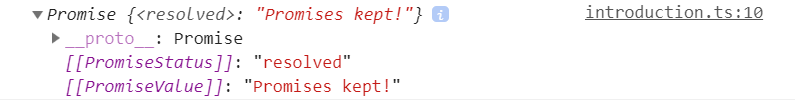
\includegraphics{promise-beispiel-1}
\caption{Promises haben einen Status und einen Wert}
\end{figure}

\begin{figure}[H]
\begin{lstlisting}
export interface FakeHttpResponse {
    code: string;
    message: string;
}

const second = new Promise<FakeHttpResponse>(function(resolve, reject) {
    setTimeout(() => {
        resolve({
            code: '200',
            message: 'Promise kept!'
        });
    }, 10 * 1000);
});

console.log(second);
setTimeout(() => console.log(second), 10 * 1000);
\end{lstlisting}
\end{figure}

\noindent
Im oberen Beispiel wird der Promise vorbehaltlos nach zehn Sekunden aufgelöst, solange ist der Status ausstehend (pending). Nachdem der Promise aufgelöst wurde, werden Status und Wert aktualisiert. Dabei können nicht nur primitive Typen wie number, boolean oder string zurückgegeben werden, sondern auch Objekt-Typen und komplexe Typen. Mit anderen Worten: Promises sind generisch.

\begin{figure}[H]
\centering
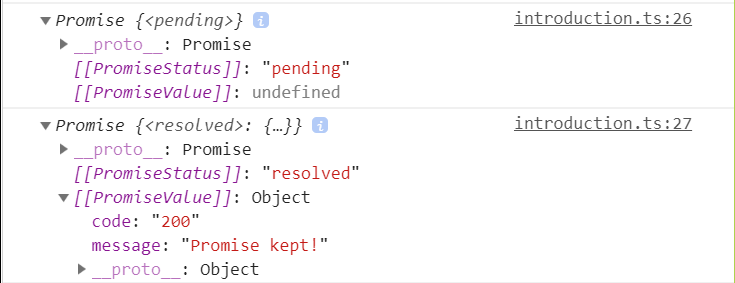
\includegraphics{promise-beispiel-2}
\caption{Promise hat anfangs den Status \glqq{}ausstehend\grqq{}}
\end{figure}

\noindent
Wie man nun gesehen hat kann der Promise-Status entweder auf \textbf{pending}, \textbf{resolved} oder \textbf{rejected} laufen. Im Status pending ist der Ausgang der Aktion noch ungewiss und deshalb der Promise-Wert undefined. Ändert sich der Status bzw. ist die Aktion zum Promise eingeschlagen oder fehlgeschlagen, ist der Status \textbf{settled}. Grundsätzlich läuft ein Promise also vom pending in den settled Status. In der nächsten Sektion wird auf das Verarbeiten von Promises näher eingegangen.

\subsubsection{Verarbeiten von Promises}

Nochmal zur Wiederholung: Ein Promise-Objekt repräsentiert das eventuelle Einschlagen oder Fehlschlagen einer asynchronen Operation, einschließlich des eingetroffenen Wertes. Ein solches Objekt bietet \textbf{statische} Methoden und \textbf{Prototyp}-Methoden. Die statischen Methoden können unabhängig von der Instanz aufgerufen werden, während die Prototyp-Methoden nur mit einer Instanz eines Promise-Objekts aufgerufen werden können. Es gibt drei Prototyp-Methoden. Alle der folgenden Methoden lassen sich unter einem Promise-Event einordnen.
Zur Wiederholung der verschiedenen Promise-Events:

\begin{itemize} 
\item Pending: Der Ausgang des Promises ist noch(!) ungewiss.
\item Resolved: Die Aktion, die zum Promise verlief, schlug ein.
\item Rejected: Die Aktion, die zum Promise verlief, schlug fehl.
\item Settled: Die Aktion ist entweder fehlgeschlagen oder eingeschlagen - jedoch abgeschlossen.
\end{itemize}

\noindent
Eine oder mehrere der drei Prototyp-Methoden werden aufgerufen wenn ein Promise in den settled Zustand übergelaufen ist:

\begin{description}

\begin{figure}[H]
\item \begin{lstlisting}
Promise.prototype.catch(onRejected)
\end{lstlisting}
\end{figure}

\begin{figure}[H]
\item \begin{lstlisting}
Promise.prototype.then(onFulfilled, onRejected)
\end{lstlisting}
\end{figure}
 
\begin{figure}[H]
\item \begin{lstlisting} 
Promise.prototype.finally(onFinally)
\end{lstlisting}
\end{figure}
 
\end{description}

\noindent
Die untenstehende Grafik zeigt den Ablauf für das Eintreten der Events und wann die Methoden \textbf{then()} und \textbf{catch()} genutzt werden. Da beide Methoden ein Promise-Objekt zurückgeben, können Promises reibungslos aneinandergekettet werden. Wenn \textbf{finally} an ein Promise Objekt angebunden wird, wird diese Callback-Funktion in jedem Fall aufgerufen, wenn der Promise in den settled Zustand eingetreten ist, unabhängig davon ob der Promise \textbf{eingeschlagen} oder \textbf{fehlgeschlagen} ist.


\begin{figure}[H]
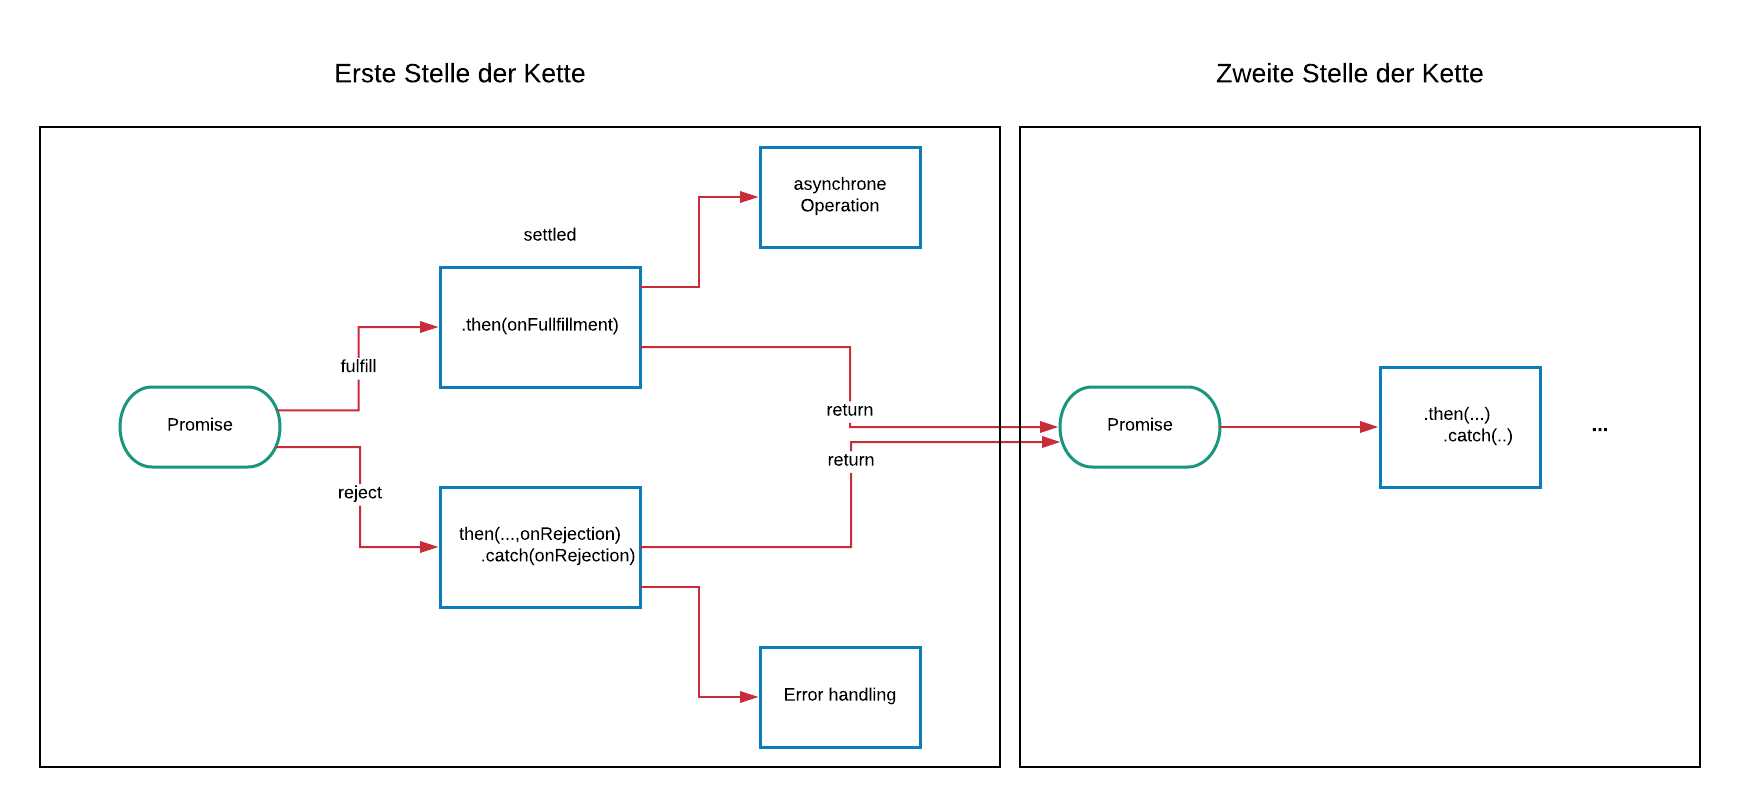
\includegraphics[width=12cm, height=6cm]{Promises-workflow}
\caption{Ablauf eines Promise-Operation \cite{promise-executor}}
\end{figure}

\noindent
Dabei kann die then() Methode zwei Argumente als Parameter entgegennehmen - einen für das einschlagen der Operation und einen für das fehlschlagen. Ein Beispiel dafür wäre:

\begin{figure}[H]
\begin{lstlisting}
get('story.json').then(function(response) {
  console.log("Success!", response);
}, function(error) {
  console.log("Failed!", error);
})
\end{lstlisting}
\caption{Error-Handling ohne catch. \cite{callback-vs-promises}}
\end{figure}

\begin{figure}[H]
\begin{lstlisting}
get('story.json').then(function(response) {
  console.log("Success!", response);
}).catch(function(error) {
  console.log("Failed!", error);
})
\end{lstlisting}
\caption{Error-Handling mit catch. \cite{callback-vs-promises}}
\end{figure}

\noindent
Im Gegensatz zur oberen Variante führt die catch() Methode keine zusätzlichen Operationen aus. Sie macht den Code lediglich semantisch lesbarer. Wichtig zu beachten ist, dass innerhalb einer Executor-Funktion \textbf{niemals} beide Argumente gemeinsam eintreffen können. Sie verhalten sich exklusiv. Deshalb ist das letztere Beispiel im Verhalten vergleichbar mit diesem Beispiel:

\begin{figure}[H]
\begin{lstlisting}
get('story.json').then(function(response) {
  console.log("Success!", response);
}).then(undefined, function(error) {
  console.log("Failed!", error);
})
\end{lstlisting}
\end{figure}

\noindent
Der Unterschied ist minimal, aber extrem hilfreich. Promise-Fehlschläge gelangen bei der nächsten then Methode in den fehlgeschlagen Callback weiter oder in die catch Methode(,wenn vorhanden). Mit then(func1, func2) wird entweder die erste oder die zweite Funktion aufgerufen, aber niemals beide. Jedoch mit then(func1).catch(func2) werden beide Callbacks aufgerufen, sollte die erste Funktion fehlschlagen. Dies ist nur Möglich, da die Funktionen in unterschiedlichen Stellen der Verkettung liegen. Neben den Prototyp-Methoden gibt es, wie bereits erwähnt, die statischen Methoden. Diese bestehen aus vier Methoden:

\begin{itemize}
\item Promise.resolve()
\item Promise.reject()
\item Promise.race()
\item Promise.all()
\end{itemize}

\noindent
Die ersten beiden Methoden werden genutzt um einen eingeschlagenen oder fehlgeschlagenen Promises zu simulieren:

\begin{figure}[H]
\begin{lstlisting}
const third = Promise.reject('I reject on purpose!');

third.catch(function(err: string) {
    console.log('Reason of failure: ' + err);
});
\end{lstlisting}
\caption{introduction.ts}
\end{figure}

\noindent
Die anderen beiden Methoden helfen Promises leichter zu verarbeiten. Beispielsweise, wenn es darum geht multiple Promises auszuführen, hat man entweder die Wahl die Promise-Verkettung zu nutzen oder die Promises in einem Array zu lagern und dann die nötigen Aktionen mit der Sammlung von Promises auszuführen. In dem nächsten Beispiel wird die \textbf{Promise-Verkettung}, \textbf{Promise.all()} und \textbf{Promise.race()} gegenübergestellt.Vor dem Ausführen des Beispiels muss folgend konfiguriert werden:

 \begin{center}
     Promises-vs.-Observables$\,\to\,$ webpack.config.js
 \end{center}

\begin{figure}[H]
\begin{lstlisting}
module.exports = {
    mode: 'development',
    entry: './src/modules/modules/stories.ts',
    ...
}
\end{lstlisting}
\end{figure}


\begin{figure}[H]
\begin{lstlisting}
export interface Post {
    userId: string;
    id: string;
    title: string;
    body: string;
}

export class HTTP {

    public makeRequest(url: string): Promise<XMLHttpRequestResponseType | string> {
        return new Promise((resolve, reject) => {
            const req = new XMLHttpRequest();
            req.open('GET', url);

            req.onload = () => {
                if (req.status === 200) {
                    this.fakeLatency(3000 * Math.random())
                        .then(() => resolve(req.response));
                } else {
                    reject(Error(req.statusText));
                }
            };

            req.onerror = () => {
                reject(Error('Network Error'));
            };

            req.send();
        });
    }

    private fakeLatency(ms: number) {
        return new Promise((resolve) =>
            setTimeout(resolve, ms));
    }
}
\end{lstlisting}
\end{figure}

\begin{figure}[H]
\begin{lstlisting}
class Story extends HTTP {

    public static BASE_URL = 'https://jsonplaceholder.typicode.com/';
    public spinnerElement: HTMLElement = document.createElement('div');
    public storyElement: HTMLElement = document.createElement('div');

    constructor() {
        super();
        this.spinnerElement.innerHTML =
            `<svg class="spinner" viewBox="0 0 100 100" width="20" height="20">
                <circle cx="50" cy="50" r="42" transform="rotate(-90,50,50)" />
             </svg>`;
    }

    public getAllStories(): Promise<XMLHttpRequestResponseType | string> {
        const relativeUrl: string = 'posts';
        return this.makeRequest(Story.BASE_URL + relativeUrl);
    }

    // Range of possible chapters: 0 < chapter <= 99
    public getChapter(chapter: number): Promise<XMLHttpRequestResponseType | string> {
        return this.makeRequest(`${Story.BASE_URL}posts/${chapter.toString()}`);
    }

\end{lstlisting}
\end{figure}
\begin{figure}[H]
\begin{lstlisting}
    public spawn(result: XMLHttpRequestResponseType): void {
        let posts = JSON.parse(result);
        if (posts instanceof Array === false) {
            posts = [posts] as Post[];
        }
        for (const post of posts) {
            this.storyElement.innerHTML +=
                `<h1>${post.title}</h1>
                    <div class="story-info"><i>ID: Post-${post.id}</i></div>
                <div><p>${post.body}.</p></div>`;
        }
    }

    public displayFinished() {
        const done: Node = document.createElement('div');
        done.textContent = 'All done!';
        document.body.appendChild(done);
    }
}

const story = new Story();
document.body.appendChild(story.storyElement);
document.body.appendChild(story.spinnerElement);
\end{lstlisting}
\end{figure}

\noindent
Dieses Beispiel kommt einem praktischen Anwendungsfall relativ nahe. Die Klasse \textbf{HTTP} stellt mit  \textbf{makeRequest()} eine Methode zur Verfügung, die eine HTTP-Anfrage gegen einen übergebenen Endpunkt macht. Die Methode \textbf{fakeLatency()} simuliert eine Verzögerung der Datenübertragung, wie es sie unter Anderem auch auf dem mobile Internet gibt. Mit der \textbf{Story} Klasse wird zunächst ein Endpunkt für die Datenabfrage definiert. Hierbei handelt es sich um JSONPlaceholder, eine Open Source Endstelle die Beispieldaten für das Prototyping oder zum Testen zur Verfügung stellt. Darüberhinaus werden mit \textbf{getAllStories()} und \textbf{getChapter()} zwei Methoden definiert, die eine Anfrage gegen zwei verschiedene Endpunkte machen.  Sollte ein Anforderungsfall sein alle Stories aufeinmal anzuzeigen, würde der Code Hierfür wie folgt aussehen:

\begin{figure}[H]
\begin{lstlisting}
story.getAllStories()
    .then((response: XMLHttpRequestResponseType) => story.spawn(response))
    .finally(() => {
        story.displayFinished();
        story.spinnerElement.style.display = 'none';
    });
\end{lstlisting}
\end{figure}

\noindent
Hier werden zunächst alle Kapitel mit einem einzigen Aufruf am Endpunkt angefragt und daraufhin im Browser abgebildet. Ist der Promise in den settled Zustand angelangt, wird mit finally der Lade-Icon ausgeblendet und eine Nachricht angezeigt, dass alle Stories abgebildet wurden. Sollte jedoch ein Anwendungsfall sein, dass nur fünf Stories im Browser angezeigt werden sollen, könnte der Code hierfür so aussehen: 

\begin{figure}[H]
\begin{lstlisting}
story.getChapter(1)
    .then((response1: XMLHttpRequestResponseType) => {
        story.spawn(response1);
    })
    .then(() => story.getChapter(2)
        .then((response2: XMLHttpRequestResponseType) => {
            story.spawn(response2);
        }))
    .then(() => story.getChapter(3)
        .then((response3: XMLHttpRequestResponseType) => {
            story.spawn(response3);
        }))
    .then(() => story.getChapter(4)
        .then((response4: XMLHttpRequestResponseType) => {
            story.spawn(response4);
        }))
    .then(() => story.getChapter(5)
        .then((response5: XMLHttpRequestResponseType) => {
            story.spawn(response5);
        }))
    .finally(() => {
        story.displayFinished();
        story.spinnerElement.style.display = 'none';
    });
\end{lstlisting}
\end{figure}

\noindent
Mit diesem Code-Beispiel wird schnell Klar, dass eine Promise-Verkettung mit mehr als zwei Ketten unübersichtlich ist. In diesem Fall werden fünf Kapitel nacheinander angefragt und im Browser angezeigt. Da die Aufrufe in dem verkettetem Konstrukt voneinander abhängig sind, addiert sich die Zeit die gebraucht wird, um ein Kapitel anzufragen und abzubilden. Sind die Kapitel unabhängig voneinander und spielt die Reihenfolge zur Darstellung keine Rolle, dann gibt es eine zweite Variante: 

\begin{figure}[H]
\begin{lstlisting}
const promises: Array<Promise<void>> = [];

for (const n of [1, 2, 3, 4, 5]) {
    promises.push(story.getChapter(n)
        .then((response: XMLHttpRequestResponseType) => {
            story.spawn(response);
        }));
}

Promise.all(promises).finally(() => {
    story.displayFinished();
    story.spinnerElement.style.display = 'none';
});
\end{lstlisting}
\end{figure}

\noindent
Promise.all() gibt ein einzelnes Promise zurück, dass einschlägt wenn alle Promises innerhalb des übergebenen Promise-Arrays einschlagen sind oder das übergebene Argument keine Promises enthält. Die Promises werden nach der Reihenfolge ihres Einschlagens aufgerufen.

\begin{figure}[H]
\centering
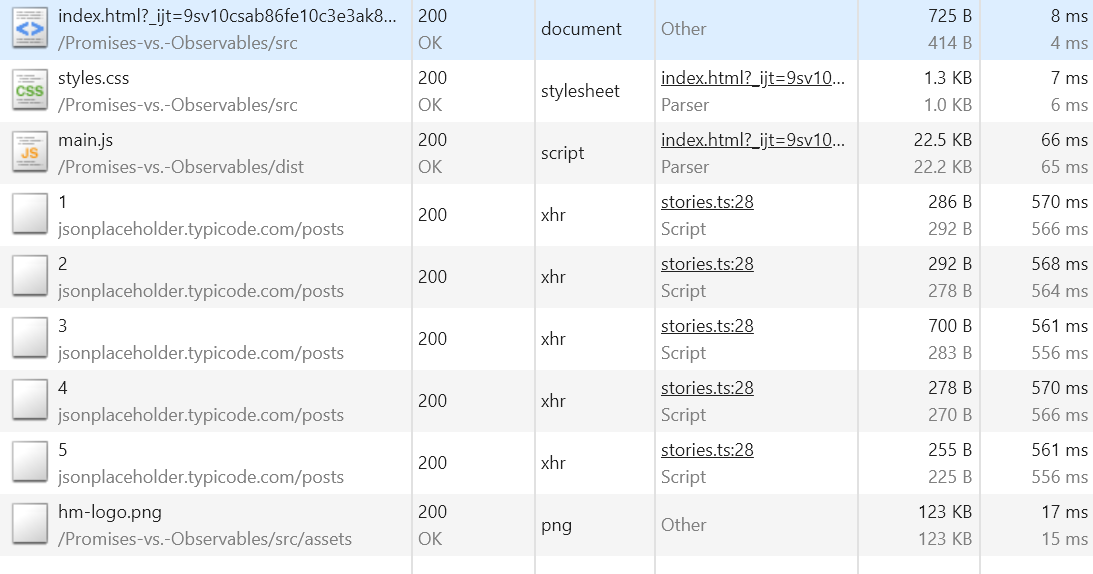
\includegraphics[width=12cm]{promises-zeitstrahl}
\caption{Die Nachrichten werden in der Reihenfolge: 3, 5, 2, 1 und 4 abgebildet.}
\end{figure}

\noindent
Sollte ein Promise fehlschlagen, wird dieser Ebenfalls fehlschlagen mit der Fehlernachricht des ersten fehlgeschlagenen Promise.\cite{promise-executor} Dabei ist zu beachten, dass die Promises parallel voneinander ausgeführt werden. Dagegen wird die nächste Methode verhältnismäßig seltener genutzt. Promise.race() gibt ein Promise zurück, dass einschlägt oder fehlschlägt, sobald das erste Promise des Übergebenen Promise-Arrays einschlägt oder fehlschlägt.\cite{versprechen}

\begin{figure}[H]
\begin{lstlisting}
Promise.race(promises).finally(() => {
    story.displayFinished();
    story.spinnerElement.style.display = 'none';
});
\end{lstlisting}
\caption{Es wird nur ein Kapitel mit der Nachricht \glqq All done!\grqq{} angezeigt.}
\end{figure}

 \noindent
 Als Faustregel für Promises sollte beachtet werden, dass sie nur für einmalig entstehende asynchrone Events genutzt werden sollten. Resolve() wird mit der then() Methode verarbeitet und reject() mit der catch() Methode gefangen. Finally() sollte nur genutzt werden, wenn eine Aktion unabhängig von beiden Events eintreten soll. Der zurückgegebene Typ einer Promise Methode ist immer ein Promise-Objekt, unabhängig davon ob es sich um eine statische- oder einer Prototyp-Methode handelt. Promises bieten mit Promise.all() und Promise.race() Hilfemethoden an, um Promise leichter zu verarbeiten.

\subsection{Async await}
**Funktionsweise und Vorteile**

\begin{enumerate} 
\item Source code Beispiel zeigen mit async await
\item Wie wandle ich z.b. eine verkettete (unlesbare) Promise-Verkettung in async await um 
\item Gegenüberstellung
\end{enumerate}


